\section{Grundlagen}\label{sec:Grundlagen}
\subsection{Quantenpunkte}
Ein Quantenpunkt \cite{quantum_dot} ist eine Materialstruktur die meistens aus Halbleitern besteht. Dabei wird die Beweglichkeit der Ladungsträger, Löcher und Elektronen, in allen drei Raumdimensionen eingeschränkt. 
Dazu wird oft eine Halbleiterheterostruktur verwendet und an den Grenzflächen zwischen den unterschiedlichen Halbleitern das zweidimensionale Elektronengas  auf null Dimensionen eingeschränkt. Diese Einschränkung kann durch Metallelektroden gemacht werden.
Die Materialstruktur ist also nulldiumensional, daher auch der Name Quantenpunkt.  Durch die Beschränkung sind die Energiezustände nicht mehr kontinuierlich, sondern diskret. Die Eigenschaften sind deshalb ähnlich wie bei einzelnen Atomen. 
Die Elektronen haben dann die Möglichkeit durch Tunnelprozesse von einem Quantenpunkt zum nächsten zu gelangen. 
Der Unterschied zu den Atomen ist, dass bei Quantenpunkten die elektronischen und optischen Eigenschaften im bedingtem Rahmen  selber festgelegt werden können. 
Für die Herstellung von Quantenpunkten gibt es verschiedene Verfahren. Bei der Nasschemischen Methode liegen die Nanopartikel als Kolloide in einer Suspension vor. Bei der selbstorganisierten Molekularstrukturepitaxie entstehen Quantenpunkte an der Grenzfläche zwischen dünnen Schichten von unterschiedlichen Halbleitern. Die Ursache für die selbstorganisierten Quantenpunkte liegt bei den unterschiedlichen Gitterkonstanten von den unterschiedlichen Halbleitern. Daduch kommt es zu Verspannugen und es ist energetisch günstiger dass sich die  kleine Erhebungen in der Quantenpunktschicht bilden. Ein weiteres Verfahren ist die Lithographie, bei der die Quantenpunkte mittels Elektronenstrahlen oder ähnlichem auf ein Substrat   \glqq geschrieben\grqq{} werden. Danach müssen die Quantenpunkte noch \glqq freigelegt\grqq{} werden. \\
Damit die Quantenpunkte auch quantenmechanische Eigenschaften aufweisen, muss die Grö{\ss}e der Quantenpunkte in dem Bereich der De-Broglie-Wellenlänge liegen.  Mit den Ausdrücken für die Energie $ E = \mathrm{k}_{\mathrm{B}} T$ und $ E = p^2/(2m_{\mathrm{e}}^\star)$ ergibt sich
\begin{equation}
\lambda = \frac{h}{p} = \frac{h}{\sqrt{2m_{\mathrm{e}}^\star \mathrm{k}_{\mathrm{B}} T}} \approx 7.6\ \mathrm{nm},
\end{equation}
 wobei für die Temperatur $T=300$ K angenommen wird. Dieser Wert ist nur eine Näherung, da die effektive Masse der Elektronen $m_{\mathrm{e}}^\star$ materialspezifisch ist. Ein Quantenpunkt kann aus $10^3$ bis $10^9$ Atomen bestehen. \\
 
\subsection{Modelle für Quantenpunkte}
Das Verhältnis von der Höhe (z-Richtung) zur lateralen Ausdehnung  (x und y Richtung) ist klein für selbstorganisiertes Wachstum. Deshalb gibt es in dem Potential des Quantenpunktes nur einen Zustand. Die laterale Ausdehnung kann man als eine zweidiemsionales System betrachten. Die Wechselwirkung von einzelnen Quantenpunkten muss bei der Beschreibung nicht berücksichtigt werden, da der Abstand deutlich grö{\ss}er ist als die laterale Ausdehnung der Quantenpunkte. 
Das einfachste Modell eines Quantenpunktes ist ein Potentialtopf mit unendlichen hohen Wänden. Ein verbessertes Modell ist die Verwendung von endlich hohen Wänden, die die Unterschiede zwischen dem Quantenpunkt und der Umgebung beschreiben. Ein besseres Modell ist ein zweidimensionaler harmonischer Oszillator \cite{Nolting} für die laterale Ausdehnung. Nach der Abseparierung der z-Richtung lautet der Hamiltonian
\begin{equation}  
H = \frac{p_\mathrm{x}^2}{2 m^\star} + \frac{p_\mathrm{y}^2}{2 m^\star} + \frac{1}{2} m^\star \omega^2 x^2 + \frac{1}{2} m^\star \omega^2 y^2. 
\end{equation} 
Die bekannten Energieeigenwerte davon sind 
\begin{equation}
E_{\mathrm{x,y}} = \hbar \omega (2n +|l| +1)
\end{equation}
wobei die Hauptquantenzahl die Werte $n = 0,1,2, ...$ und die Nebenquantenzahl die Werte $l = 0, \pm1, \pm2, ...$ annehmen kann. 
Die Eigenfunktionen bestehen aus den Hermite Polynomen. Analog zur Atomphyisk kann der Parameter 
\begin{equation}
S = 2n +|l| = 0,1,2, ...
\end{equation}
definiert werden. Dies entspricht den Oribitalen (s,p,d,f) in Atomen \cite{Haken_Wolf}. 
Der Grundzustand ist somit das s-Orbital mit $S = 0$. 
Für die Entartung $d$ ergibt sich 
\begin{equation}
d = 2(S+1),
\end{equation}
wobei der Faktor 2 von der Spinentartung kommt. Es kann gezeigt werden, das die Quantenzahlen bei den Übergängen erhalten bleiben müssen.  Es gilt somit die Auswahlregel $\Delta S =0$. 
\subsection{Fluoreszenz}
Durch das Bescheinen eines Quantenpunktes mit einem Laser, tritt Fluoreszenz auf. Fluoreszenz ist die spontane Emission von Licht durch einen Elektronenübergang. Dafür ist es notwendig, das die Photonen, die vom Laser emmitiert werden, ausreichend  Energie haben um ein Elektron in das Leitungsband anzuheben. Dabei entsteht ein Loch in dem Valenzband. Dabei könnte grundsätzlich  ein gebundenes oder ein ungebundenes Elektronen-Loch-Paar entstehen. 
In einem Quantenpunkt treten nur gebundene Elektronen-Loch-Paare auf, da der zu Verfügung stehende  Raum in einem Quantenpunkt begrenzt ist.
 Das gebundene Elektronen-Loch-Paar wird als Exziton bezeichnet. Dabei können auch Multiexzitonen auftreten. Bei einem Biexziton sind zum Beispiel zwei Elektronen und zwei Löcher beteiligt. 
 Exzitonen kann man unterteilen in helle und dunkle Exzitonen. 
 Helle Exzitonen  sind optisch zugänglich und dunkle Exzitonen sind es nicht. 
 Das bedeutet, das die dunklen Exzitonen eine deutlich längere Lebensdauer haben als helle Exzitonen. 
 Das dabei von den Quantenpunkten durch Rekombination von Elektronen mit Löchern emittierte Licht, ist im Allgemeinen energieärmer als das davor absorbierte Licht. Das absorbierte Licht stammt von dem Laser. 
 Andere Verwendungsmöglichkeiten von  Quantenpunkten sind die Verwendung als Einzelphotonenquellen und als Laser.
 Ein emmitiertes Photon hat den Drehimpuls $\pm \hbar$. Bei der Emission eines Photons  mit dem Drehimpuls $+ \hbar$ muss somit der gesamte Drehimpuls um den gleichen Betrag vermindert werden und umgekehrt. Es gilt die Auswahlregel $ \Delta J = \pm 1$, wie in Abbildung \ref{fig:QP_Energien} zu sehen ist.
 \begin{figure}[H]
\centering
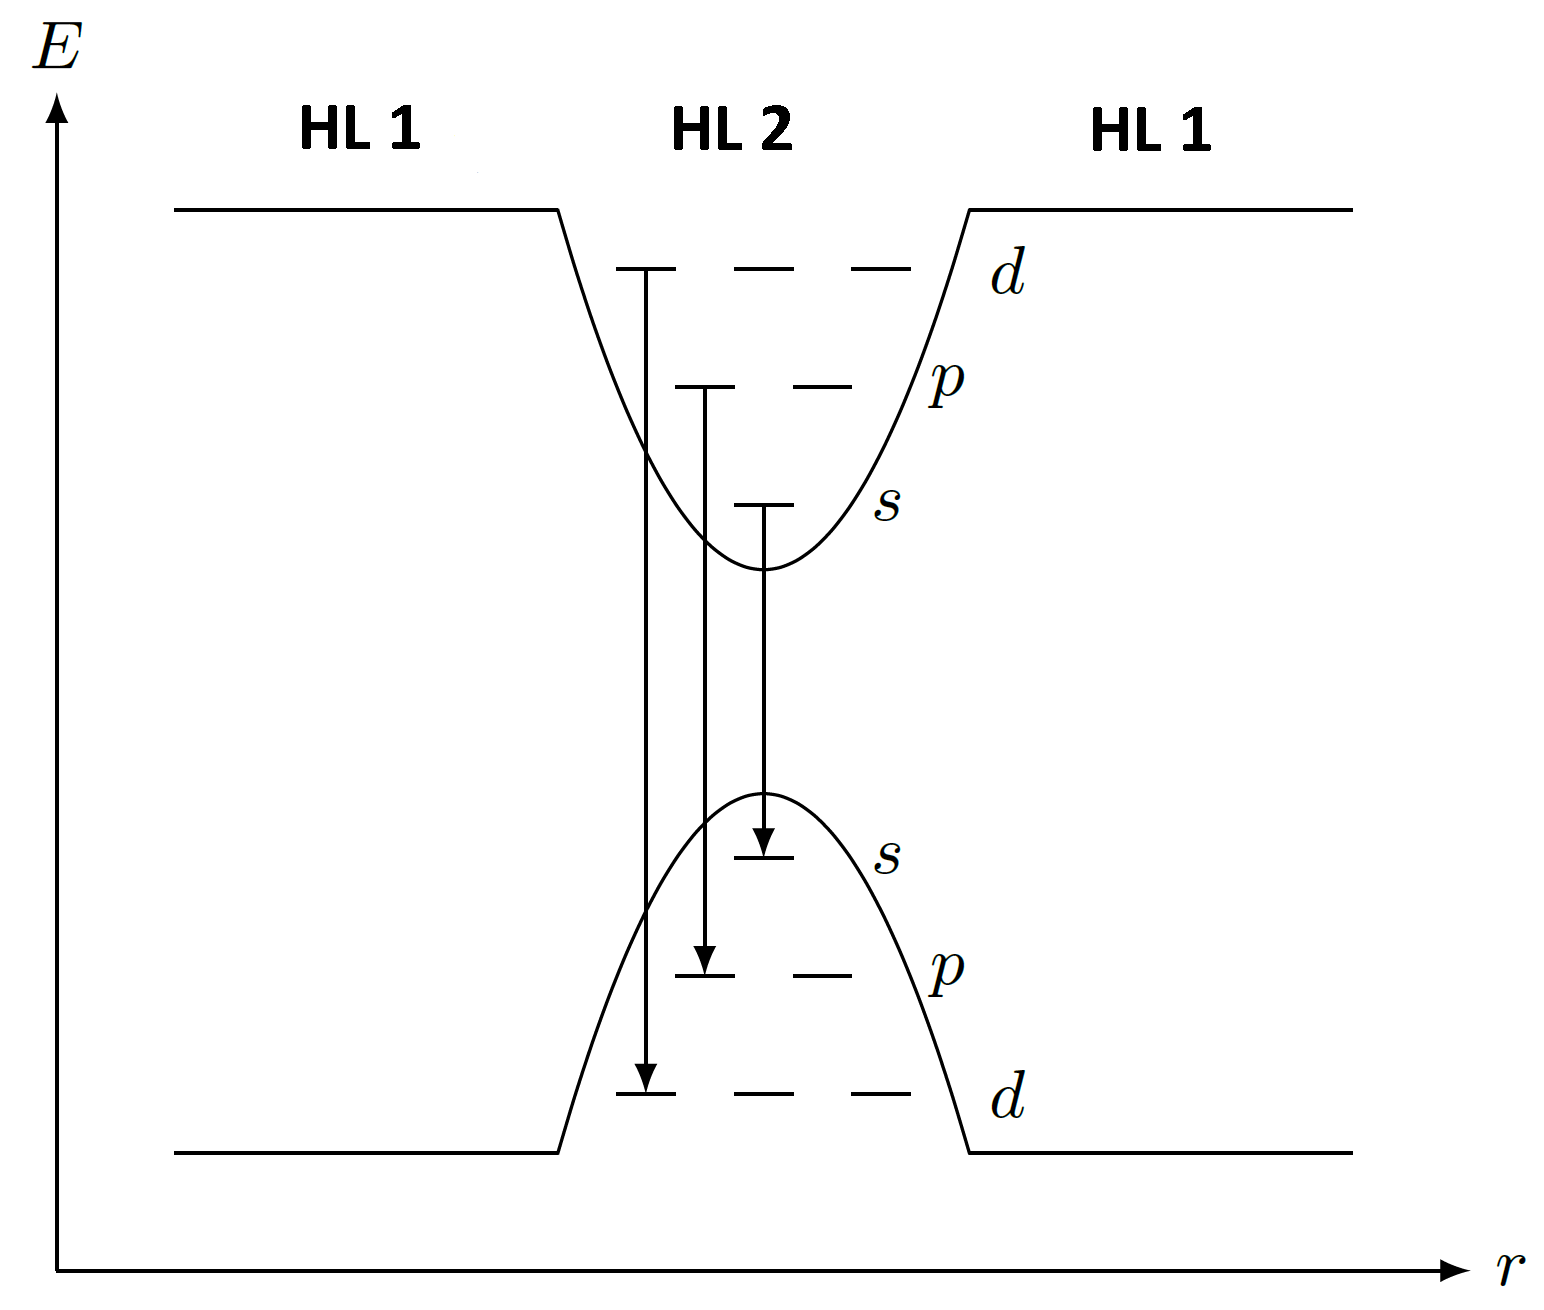
\includegraphics[scale=0.3]{QP_Energie.PNG}
\caption{Erlaubte Übergänge in einem Quantenpunkt, wobei HL1 und HL2 die Abkürzungen für die beiden unterschiedlichen Halbleiter sind.}
\label{fig:QP_Energien}
\end{figure}
\subsection{Spektrum von Quantenpunkten}
In dem Spektrum sind nicht alle erlaubten Übergänge des zweidiemsionalen harmonischen Oszillator Modells gleich strak vertreten. Die Höhe der Peaks hängt von der Entartung ab. Je grö{\ss}er die Entartung eines Zustandes ist, desto grö{\ss}er ist der Peak. Der kleinste Peak sollte deshalb von dem s-Orbital kommen. Da dies nicht der einzige auftredente Effekt ist, muss dies in einem Experiment nicht der Fall sein. Eine Ursache dafür kann die Temperatur sein. Bei höheren Temperaturen nimmt der Einfluss der Phononen zu und es sind deshalb weniger Peaks sichtbar. 
Die Ursache dafür ist das bei der Rekombination von Elektronen und Löchern die Energie an ein weiteres Elektron bzw. Loch abgegeben wird und dann mittels einer Wechselwirkung mit Phononen an das Gitter abgegeben wird.
Die Intensität des Lasers, der für die Fluoreszenz benötigt wird, verändert ebenfalls das Spektrum. Bei höheren Laserintensitäten sind mehr Peaks sichtbar. 
Bei niedrigen Laserintensitäten sind nur die niedrigeren Zustände besetzt und somit können auch nur diese zum Spektrum beitragen.
Nicht alle gemessenen Peaks stammen von dem Quantenpunkt. Es gibt zum Beispiel auch einen Peak des Substrates.
Der Laser der für die notwendigen Anregungen bei der Fluoreszenz notwendig ist, regt auch Übergänge in dem Substrat an. Nach der Lebensdauer der angeregten Zustände geht das Substrat wieder in den Zustand niedrigerer Energie über, wobei die frei werdende Energie als Photon emmitiert wird. \\
Eine Messung kann nie unter Idealbedingungen durchgeführt werden. Dadurch kommt es zu Linienverbreitungen und Linienverschiebungen. Die Peaks haben deshalb die Form einer Gau{\ss}funktion. Eine Ursache dafür ist die Unbestimmtheitsrelation. Die Lebensdauer eines angeregten Zustandes ist verknüpft mit der Unbestimmtheit ihrer Energie.  Dabei bedeutet eine kurze Lebensdauer eine gro{\ss}e Energieunbestimmtheit. Dies führt im Spektrum zur einer Linienverbreiterung.
Dieser Effekt hat aber nur einen geringen Einfluss und ist meistens geringer als die Auflösung des Spektrometers. 
Ein anderer Effekt ist die thermische Dopplerverbreitung. Durch die endliche Temperatur gibt es eine thermische Bewegung. Die Emitter bewegen sich somit relativ zum Spektrometer. Die Linien sind somit entweder Rot- oder Blauverschoben.
Bei Festkörpern ist dies nicht relevant. 
Eine weitere Liniverbreiterung kann entstehen, wenn Photonen von mehreren Quantenpunkten detektiert wird. Das gemeinsame Spektrum ist eine Gaußkurve. Die Ursache dafür ist, das bei der Herstellung es zu einer gaußförmigen Größenverteilung der Quantenpunkte kommt. Die unterschedlich großen Quantenpunkte emmitieren bei leicht unterschiedlichen Wellenlängen. 
Die Lorentzkurven der einzelnen Quantenpunkte überlagern sich und dabei entsteht eine Gaußverteilung. 
\subsection{Experimentelles}
Für die Anregung der Quantenpunkte wird ein He-Ne-Laser benutzt. Dabei handelt es sich um ein Vier-Niveau-System. 
Das Helium wird zum Pumpen verwendet. 
Als erste wird das Helium, was sich im Grundzustand befindet, mittels Elektronenströ{\ss}en angeregt. 
Danach kommt es durch Stö{\ss}e zwischen Helium und Neon zu einer Anregung von Neon. 
Das Neon kann dann Photonen emittieren. 
Dies sind die Photonen, die nacher den Laser verlassen. 
Durch Stö{\ss}e, zum Beispiel mit Wänden, gelangt Neon wieder in den Grundzustand. 
Nun beginnt alles wieder von vorne. \\
Zur Messung des Spektrums wird ein Gitterspektrometer verwendet. Dabei trifft das Licht auf ein Gitter, an dem Beugung auftritt. Diese Beugung ist abhängig von der Frequenz der Photonen. 
Das hei{\ss}t unterschiedliche Frequenzen werden unterschiedlich stark gebeugt. 
Die spektrale Verteilung der Intensität erhält man durch unterschiedliche starke räumliche Ablekung.
Aufgenommen werden nun die Photonen mit einem CCD-Sensor. 
Die Abkürzung CCD steht dabei für charge-coupled-device. 
Diese basieren auf dem inneren Photoeffekt. 
Dabei werden in einem Halbleiter Elektronen von dem Valenzband ins Leitungsband angehoben und in dem Valenzband entsteht ein Loch. 
Dabei handelt es sich um ungebundene Elektronen-Loch-Paare. 
Die Auflösung von einem Spektrometer wird durch das Rayleigh-Kriterium beschrieben. 
Das Kriterium gibt den Mindestabstand zweier Lichtquellen an, damit diese noch getrennt beobachtbar sind. Das Auflösungsvermögen $R$ ist definiert als 
\begin{equation}
R = \frac{\lambda}{\Delta \lambda} = n N,
\label{eq:Auflösung}
\end{equation}
wobei $\lambda$ die verwendete Wellenlänge ist, $\Delta \lambda$ der kleinste messbare Wellenlängenunterschied ist, $n$ die Beugungsordnung und $N$ die Gitterlinien. 
Das bedeutet, je grö{\ss}er die Anzahl der Gitterlinien und mit steigender Beugungsordnung, nimmt das Auflösungsvermögen zu. 









